\chapter{基于改进Vision Transformer骨髓血细胞检测算法设计与实现}
\section{引言}
% 研究背景,现状 挑战与本文贡献
白血病是一种人体造血系统的恶性肿瘤,在所有恶性肿瘤中占比约5\%,是我国重点防治的十大恶性肿瘤之一。
血细胞形态学检查是白血病诊断常规检查的一部分,各类骨髓血细胞经过染色后呈现出不同的形状、颜色与纹理,
这些细胞由经验丰富的病理专家识别并计数,最终根据FAB标准给出白血病类型的诊断。上述人工镜检的诊断流程存在以下不足,
人工分类计数繁琐费时,诊断结果具有较强的主观性。此外,细胞形态学人才资源紧缺,
培养精通细胞病理诊断的医师要耗费大量的时间。通过研究骨髓血细胞自动化识别技术来辅助临床诊断,可以实现诊断流程的标准化、
快速化与智能化,将医生从繁重的病理工作中解放出来,具有重要的临床意义和广阔的应用前景。

近年来,基于深度学习的方法在医学影像处理领域取得了巨大的成功,
国内外学者纷纷开始探索基于深度学习的血细胞识别方法。基于深度学习的血细胞识别方法不再需要进行复杂的血细胞特征工程
设计,直接将血细胞数据输入网络中进行端到端训练。通过优化损失函数,网络可以自动挖掘数据的潜在特征,并基于这些特征进行
预测,相比于传统识别方法具有更高的识别准确率。根据文献调研,血细胞识别算法主要基于计算机视觉领域的目标识别网络并通过迁移学习进行微调,这些识别
网络包括了ResNext、ResNet与EfficientNet等,在血细胞数据集上获得了很好的识别结果。

骨髓血细胞自动化识别是一项非常具有挑战性的任务,主要存在着以下难点:(1)缺少大规模的骨髓血细胞识别任务数据集,
不同批次的骨髓血细胞存在染色、光照等差异,导致切片图像外观、颜色变化的多样性。
(2)各类骨髓血细胞在人体中的所占比例不同,导致数据集中各个类别样本数量分布不均衡,
数量较少类别的骨髓血细胞难以有效的进行特征学习。
(3)骨髓血细胞种类繁多,例如粒细胞有原始、早幼、中幼与晚幼等阶段,
相邻发育阶段的血细胞在形态上非常类似,骨髓血细胞子类之间差异较小增加了细粒度识别的难度。

针对骨髓血细胞识别过程中的难点,本章提出了一种基于改进Vision Transformer的骨髓血细胞识别方法。
首先,使用第四章提出的改进RetinaNet网络从图像中检测出细胞边界并进行裁剪,去除背景等干扰。
接着,本章提出一种重叠图像块划分方法将裁剪后的图像分割为多个图像块并学习嵌入向量表示。
然后,嵌入向量经过多个编码层进行特征提取。本章基于多头自注意机制提出了稀疏注意力模块,
该模块可以捕捉图像中的辨识性区域,提取图像中的细粒度特征,并将筛选后的特征输入到编码层。
最后,网络输出的分类特征用于骨髓血细胞的识别。在训练过程中,本章采用对比损失进一步增加分类特征的类内一致性与类间差异性。
为了进一步解决骨髓血细胞类内差异性小的问题,本章提出了了一种分级的骨髓血细胞识别算法,先由第一级网络识别大类血细胞,
再由二级网络对子类进行识别。最后,在邃蓝智能骨髓血细胞数据集与开源的慕尼黑血细胞形态学数据集实验结果表明,
我们提出的方法具有良好的精细分类性能,相比于其他识别方法具有更高的识别准确率

\section{改进的Vision Transformer骨髓血细胞识别网络}

本文提出的基于Vision Transformer的骨髓血细胞识别网络框架如图~\ref{fig:vit}所示。
首先将输入的血细胞图像分割为$N$个$P \times P$大小的图像块,接着将图像块线性映射为序列化嵌入向量,
其次加入可学习的分类向量与位置编码信息。然后嵌入向量被输入到多个堆叠的编码模块中进行特征提取。
在最后一层编码模块前,使用辨识性区域选择模块来寻找图像中的区分性像素块并将其对应的隐含特征作为输入。
最后编码器输出的分类特征经过全连接层得到骨髓血细胞的类别概率信息。

\begin{figure} 
   \centering   
   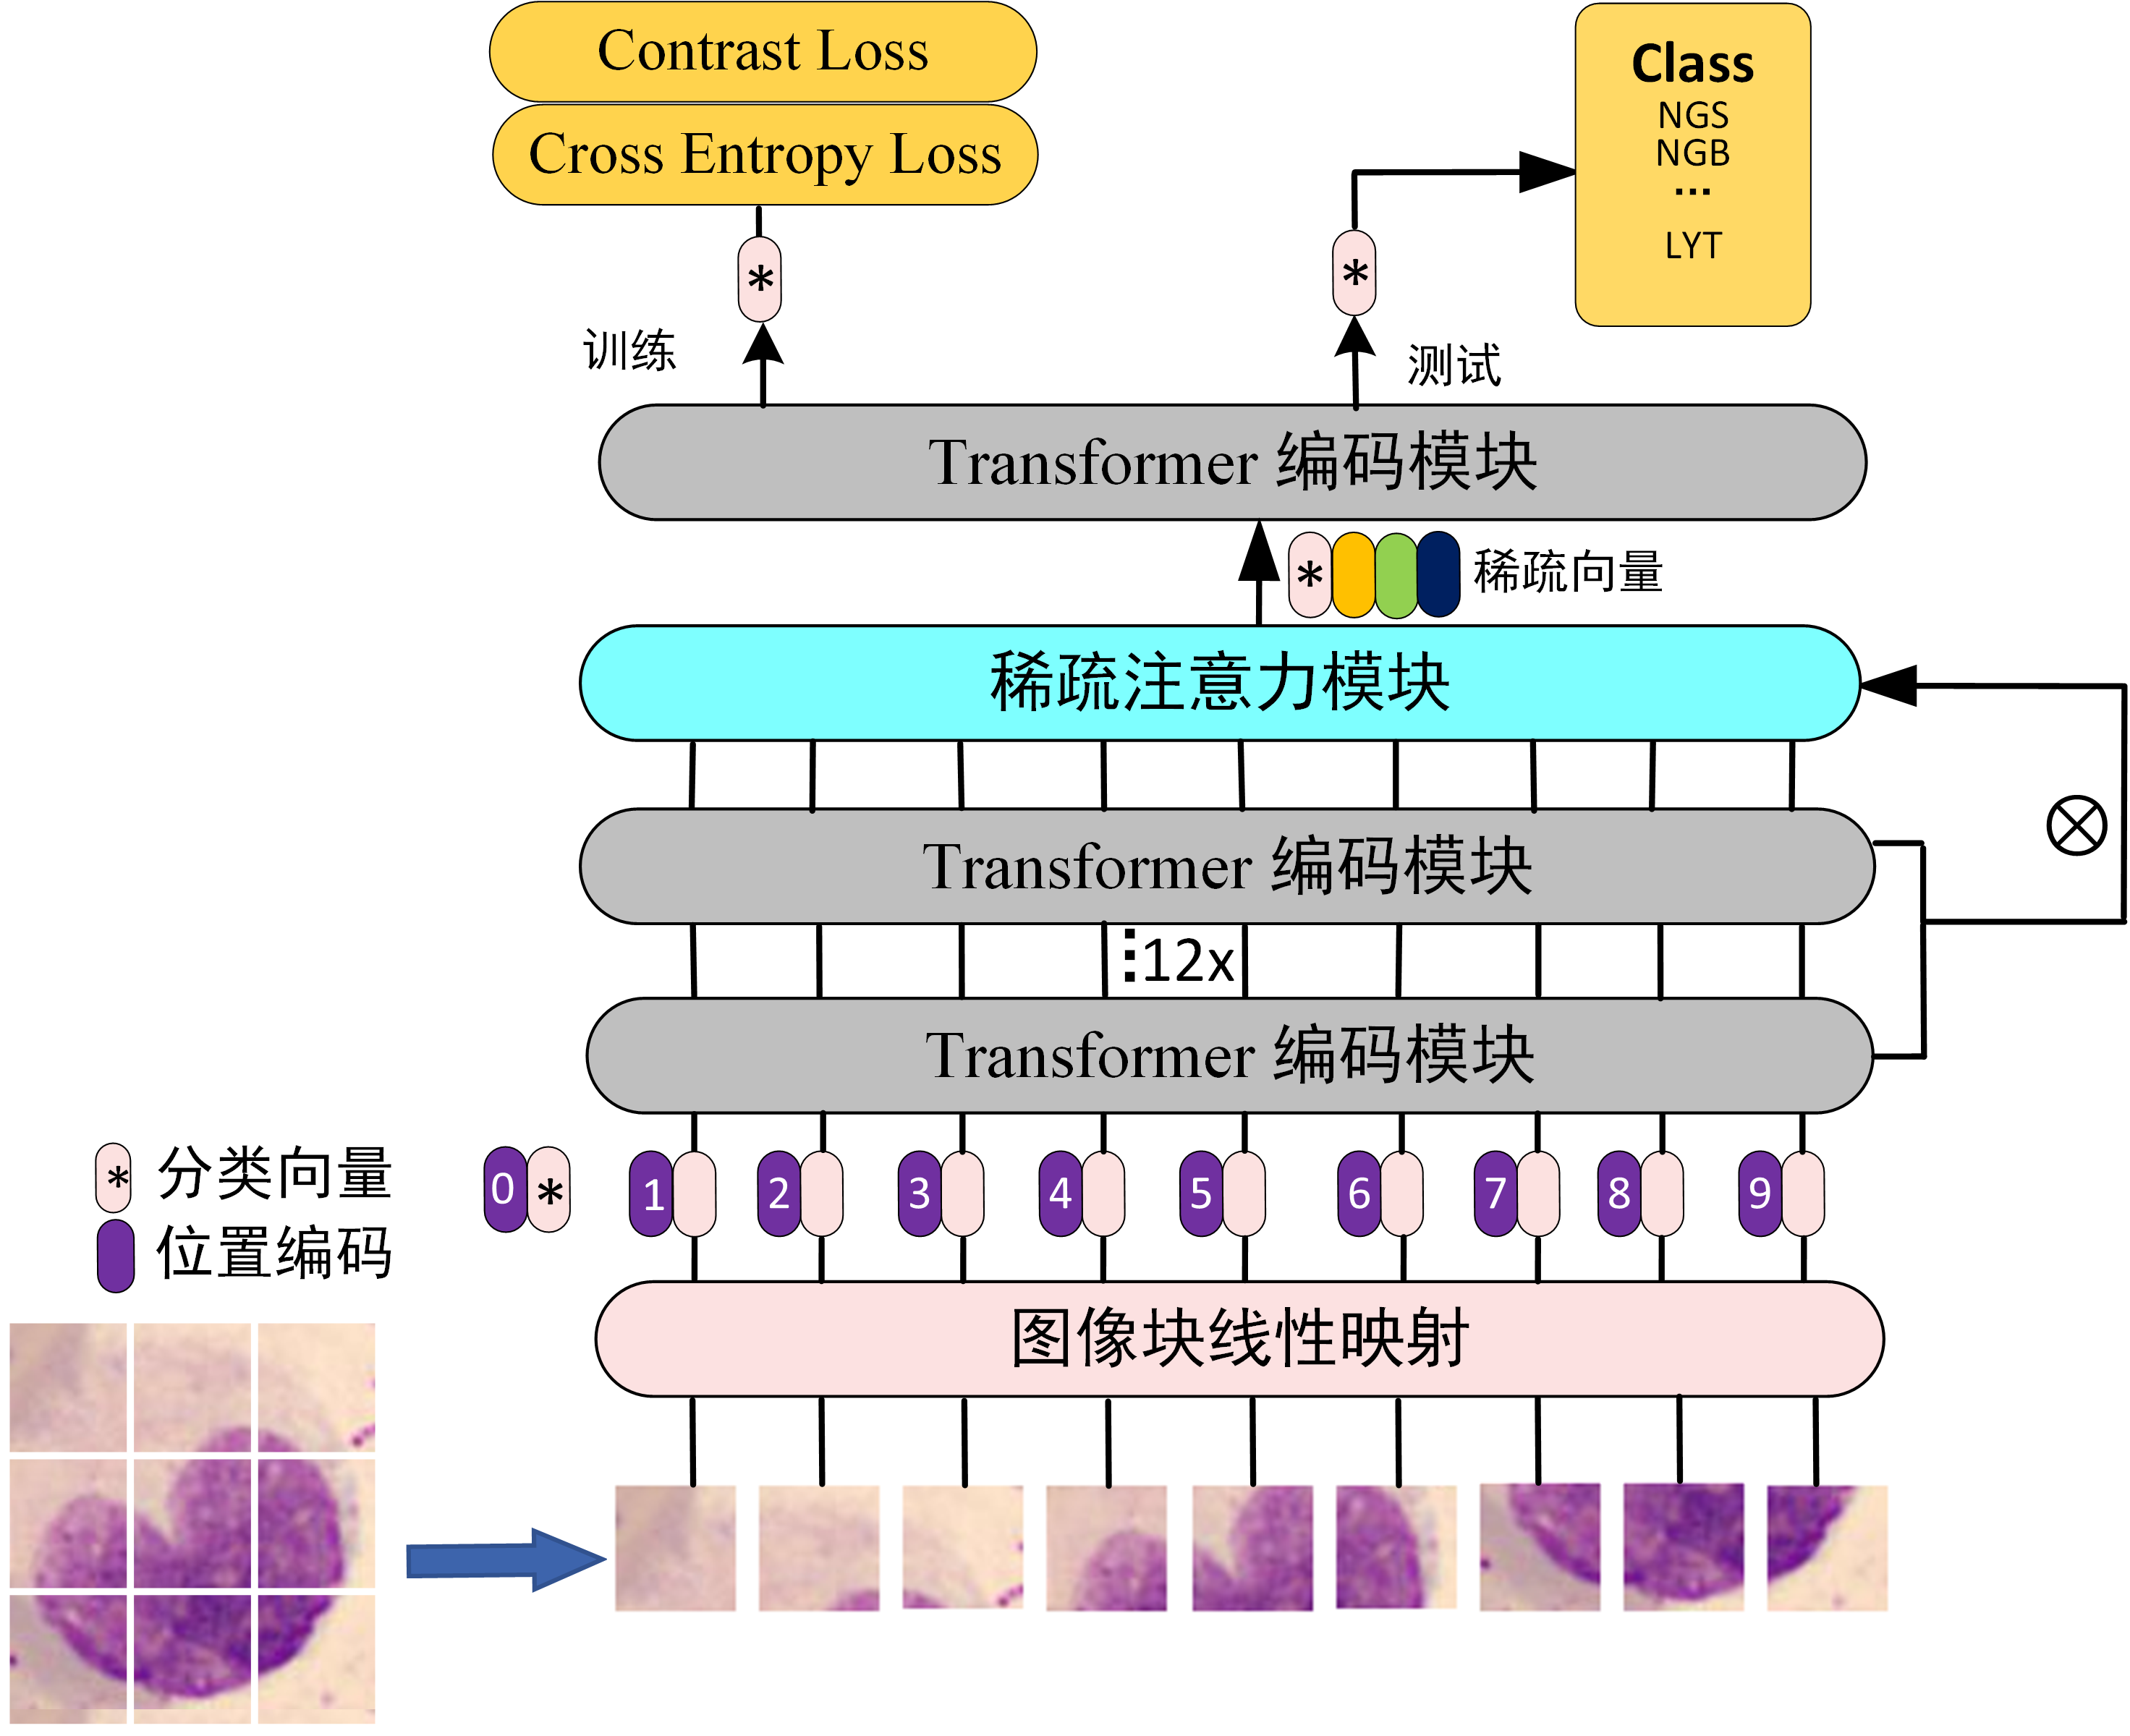
\includegraphics[width=0.9\linewidth]{transFG.png}   
   \caption{基于改进Vision Transformer骨髓血细胞识别网络结构}   
   \label{fig:vit} 
\end{figure}  

\subsection{重叠图像块划分}
Vision Transformer模型接收的输入为序列化数据,因此需要将图像划分为图像块并线性映射为序列化向量。
Vision Transformer模型将图像划分成大小为$P \times P$且互不重叠的像素块,但这样划分会破坏图像的局部结构,
例如辨识性区域被划分到两个相邻的图像块中。为避免该问题,本文采用滑动窗的方法来生成有重叠的图像块。
当输入图像的尺寸为$H \times W \times C$、图像块大小为$P$、滑动窗的步长为$S$时,图像将会被划分为$N$个像素块,
其中$N$如式~\ref{eq:embed}所示。
\begin{equation}
  n=n_{h} \times n_{w}=\left\lfloor\frac{h-p}{s}+1\right\rfloor \times\left\lfloor\frac{w-p}{s}+1\right\rfloor
  \label{eq:embed}
\end{equation}

通过滑动窗的方式,两个相邻像素块的重叠面积为$(P-S) \times P$,更好的保留了图像的局部信息。
当$S$越小,局部结构保存的越完整,但会增加序列化向量的数量导致计算开销变大。
综合利弊,在实验中将S的大小设置为$2P/3$。图像划分完成后,需要将2-D的图像块转化为1-D的序列向量,
首先将图像块展平为一组向量$x_{\mathrm{p}} \in \mathbb{R}^{N \times P^{2} \mathrm{C}}$,
然后通过线性变换将其映射到$D$的维度大小。
上述转化在具体实现上等价于对原图像进行$D$个$P×P×P^2C$x 尺寸的卷积核、步长为$2P/3$的卷积操作。
由于嵌入后的向量不包含位置信息,需要加入一个特殊的可学习位置编码。
此外还加入可学习分类向量作为最终的输出特征用于图像分类。
嵌入后的序列数据$\boldsymbol{z}_{0}$如式~\ref{eq:embed1}所示,其中$\boldsymbol{E}$为投影矩阵、$\boldsymbol{E}_{\mathrm{pos}}$为位置编码、$\boldsymbol{x}_{\text {class }}$为分类向量。
\begin{equation}
    \boldsymbol{z}_{0}=\left[\boldsymbol{x}_{\text {class }} ; \boldsymbol{x}_{p}^{1} \boldsymbol{E} ; \boldsymbol{x}_{p}^{2} \boldsymbol{E} ; \cdots ; \boldsymbol{x}_{p}^{N} \boldsymbol{E}\right]+\boldsymbol{E}_{\mathrm{pos}}
    \label{eq:embed1}
\end{equation}


\subsection{编码层}
\subsection{辨识性区域选择模块}
\subsection{损失函数}

\section{基于分级网络的骨髓血细胞识别方法}

\section{算法实现与实验结果分析}
\subsection{实验环境}
\subsection{消融实验}
\subsection{分级网络性能分析}
\section{小结}